\chapter{CARDIAC STRUCTURE SEGMENTATION USING AN ENHANCED U-NET WITH FUZZY POOLING}
\label{chap:4}

\section{Overview}
\label{sec:ch4-intro-overview}

This chapter presents the development and evaluation of the proposed cardiac structure segmentation framework, which constitutes the first stage of the deep learning framework for myocardial infarction assessment developed in this dissertation. Specifically, this chapter investigates the effects of activation function selection and fuzzy pooling layer configuration on cardiac structure segmentation performance using cine cardiac magnetic resonance images. The resulting anatomical representations provide the foundation for the subsequent investigation of myocardium segmentation and myocardial scar assessment presented in the following chapters.

Cardiovascular disease remains one of the leading causes of mortality worldwide and continues to impose a substantial clinical and socioeconomic burden despite significant advances in diagnostic and therapeutic technologies \citep{Tsao2022,WHO2021}. Accurate assessment of cardiac morphology and function is therefore essential for early diagnosis, treatment planning, and long-term monitoring of patients with various cardiovascular disorders. Among available imaging modalities, CMR has become the clinical reference standard because it provides high spatial resolution, excellent soft tissue contrast, and comprehensive visualization of cardiac anatomy and ventricular function without ionizing radiation \citep{Agrawal2020}.

Quantitative clinical parameters derived from CMR, including ventricular volume, myocardial mass, stroke volume, and ejection fraction, are obtained through the segmentation of the left ventricle (LV), right ventricle (RV), and myocardium (MYO) across the cardiac cycle. Consequently, accurate segmentation of these anatomical structures constitutes a fundamental prerequisite for reliable functional assessment and subsequent diagnosis. Any segmentation inaccuracies directly propagate into quantitative measurements, potentially affecting clinical interpretation and therapeutic decision-making \citep{Petitjean2011,Bernard2018}.

Although manual segmentation remains the clinical reference standard, numerous CMR image segmentation methods have been proposed to improve accuracy, efficiency, and reproducibility \citep{Petitjean2011}.

Recent advances in deep learning have substantially improved automatic medical image segmentation. Among various convolutional neural network architectures, U-Net has become one of the most widely adopted frameworks because its encoder--decoder structure, combined with skip connections, effectively integrates semantic information and fine spatial details, enabling accurate localization even with relatively limited annotated medical datasets \citep{Ronneberger2015,Siddique2021}. Consequently, numerous CMR image segmentation methods have been developed to overcome these limitations using deep learning techniques \citep{Ronneberger2015,Siddique2021}.

Despite its widespread success, the segmentation accuracy of conventional U-Net remains influenced by several architectural components. One critical component is the pooling operation applied during the encoder pathway. Conventional max pooling reduces feature-map resolution by retaining only the maximum activation within each pooling region. While this strategy effectively enlarges the receptive field and decreases computational complexity, repeated application may discard weaker activations that still contain important anatomical information, particularly around thin myocardial boundaries and low-contrast tissue interfaces \citep{Nirthika2022,Diamantis2020}. Such information loss may reduce boundary precision and adversely affect the delineation of anatomically complex cardiac structures.

Several alternative pooling strategies have therefore been proposed to preserve richer spatial representations during feature aggregation. Among these approaches, fuzzy pooling introduces fuzzy membership concepts to aggregate information from multiple activations rather than relying solely on the strongest response. By incorporating weighted contributions from neighboring activations, fuzzy pooling is expected to preserve local contextual information more effectively while reducing sensitivity to minor image variations and noise \citep{Diamantis2020}. Nevertheless, its effectiveness for multi-structure cardiac segmentation using cine cardiac MRI has not been comprehensively investigated.

Based on this research gap, this chapter develops an enhanced cardiac structure segmentation framework by integrating fuzzy pooling into the encoder pathway of the conventional U-Net architecture. Rather than introducing a completely new segmentation network, this study investigates whether improving the feature aggregation mechanism during down-sampling can preserve richer anatomical information and consequently improve the segmentation performance of the left ventricle (LV), right ventricle (RV), and myocardium (MYO) throughout the cardiac cycle.

The proposed framework is implemented using cine cardiac MRI obtained from the Automated Cardiac Diagnosis Challenge (ACDC) dataset. To ensure that the observed performance differences originate from the investigated pooling mechanism, the network architecture, activation function, optimizer, learning rate, training protocol, and evaluation metrics were maintained consistently across the experiments; the batch size followed the source-study configuration for each pooling strategy. Consequently, fuzzy pooling becomes the only architectural component evaluated against the conventional max pooling strategy under controlled experimental conditions.

The performance of the proposed framework is quantitatively evaluated using Intersection over Union (IoU) and Hausdorff Distance (HD), while qualitative assessment is performed through visual comparison of the generated segmentation masks. Furthermore, the experimental findings are analyzed to determine how feature preservation during the down-sampling process influences segmentation accuracy, boundary delineation, and anatomical consistency of cardiac structures.

This chapter presents an enhanced U-Net framework for cardiac structure segmentation by incorporating fuzzy pooling into the feature extraction process. The proposed modification aims to preserve richer anatomical information during down-sampling while maintaining the simplicity of the original U-Net architecture. The effectiveness of the proposed framework is evaluated through quantitative and qualitative analyses using cine cardiac MRI datasets. The enhanced cardiac structure segmentation established in this chapter subsequently provides the anatomical myocardium representation required for the investigations presented in Chapter V and Chapter VI.

\section{Proposed Cardiac Structure Segmentation Framework}
\label{sec:ch4-framework}

This chapter develops a cardiac structure segmentation framework by enhancing the conventional U-Net architecture with fuzzy pooling to improve cardiac structure segmentation through improved anatomical feature representation during encoder down-sampling. Rather than proposing a new segmentation network, this study investigates whether improving the feature aggregation mechanism alone is sufficient to enhance the delineation of the left ventricle, right ventricle, and myocardium from cine cardiac MRI.

As described in Chapter III, pooling operation is one of the architectural components that directly influences the quality of hierarchical feature representations learned by a convolutional neural network. Since all subsequent decoding and boundary reconstruction processes depend on the encoded feature maps, excessive information loss during down-sampling may propagate throughout the network and ultimately reduce segmentation accuracy. Therefore, this study focuses on improving feature aggregation during pooling while preserving the overall network architecture.

Accordingly, the proposed framework applies the original U-Net architecture as the segmentation backbone and replaces the conventional max pooling operation with fuzzy pooling in the encoder pathway. This modification aims to preserve richer anatomical information during feature down-sampling without altering the encoder--decoder topology, skip connections, or training strategy. Consequently, any performance differences observed in the experimental evaluation can be primarily attributed to the investigated pooling mechanism rather than to changes in network complexity or architectural design.

Figure~\ref{fig:ch4-workflow} illustrates the overall workflow of the proposed cardiac structure segmentation framework. Beginning with cine cardiac MRI acquisition, the framework performs image preprocessing, feature extraction using the enhanced U-Net architecture, cardiac structure segmentation, and quantitative performance evaluation.

\begin{figure}[htbp]
	\centering
	\fbox{\parbox{0.86\textwidth}{\centering Insert Overall workflow of the proposed enhanced U-Net framework for cardiac structure segmentation here}}
	\caption{Overall workflow of the proposed enhanced U-Net framework for cardiac structure segmentation}
	\label{fig:ch4-workflow}
\end{figure}
%\noindent\textit{Source: Author's illustration based on the proposed framework.}

As illustrated in Figure~\ref{fig:ch4-workflow}, cine cardiac MRI images are first preprocessed through image resizing and normalization before being forwarded into the segmentation network. The encoder progressively extracts hierarchical anatomical features while reducing spatial resolution. Unlike the conventional U-Net, each down-sampling stage incorporates fuzzy pooling to preserve contextual information that may otherwise be discarded during feature aggregation. The decoder subsequently reconstructs the segmentation masks by combining semantic representations from deeper layers with fine spatial information transferred through skip connections. The final output consists of pixel-wise segmentation masks corresponding to the left ventricle, right ventricle, and myocardium. These segmentation results are then quantitatively evaluated using IoU and HD.

The following sections describe each component of the proposed framework in greater detail.

\subsection{Baseline U-Net Architecture}
\label{subsec:ch4-unet}

U-Net has become one of the most widely adopted convolutional neural network architectures for cardiac structure segmentation because of its encoder--decoder design, which effectively combines high-level contextual information with fine spatial details through skip connections \citep{Ronneberger2015}. Unlike conventional convolutional neural networks designed primarily for image classification, U-Net performs dense pixel-wise prediction by integrating contextual information from multiple spatial resolutions through its encoder--decoder architecture.

The encoder gradually extracts increasingly abstract feature representations while reducing spatial resolution, enabling the network to learn high-level semantic information. Conversely, the decoder progressively restores the original image resolution and reconstructs the segmentation mask. Skip connections directly transfer fine-grained spatial information from corresponding encoder layers to decoder layers, allowing the network to recover anatomical details that may otherwise be lost during feature compression. This architectural characteristic has made U-Net one of the most successful frameworks for medical image segmentation involving complex anatomical structures with varying sizes and shapes.

The selection of U-Net in this study is further motivated by its extensive application in cardiac MRI segmentation. Previous studies have demonstrated that U-Net provides reliable segmentation of ventricular cavities and myocardial structures while maintaining relatively simple network complexity and efficient training characteristics. These advantages make U-Net an appropriate baseline architecture for investigating architectural modifications intended to improve segmentation performance without introducing additional sources of variation.

Despite these advantages, one limitation of the conventional U-Net lies in its use of max pooling throughout the encoder pathway. During each down-sampling operation, max pooling retains only the strongest activation within a local neighborhood while discarding all remaining responses. Although this mechanism effectively reduces computational complexity and enlarges the receptive field, repeated application may eliminate weaker activations that still contain meaningful anatomical information, particularly around thin myocardial boundaries or regions exhibiting subtle intensity variations \citep{Nirthika2022,Diamantis2020}.

For cardiac MRI segmentation, preserving these weak yet informative responses is particularly important because the myocardium often appears as a relatively thin ring-shaped structure whose boundaries exhibit gradual intensity transitions rather than sharp edges. Consequently, the accumulated information loss introduced by repeated max pooling may reduce boundary precision and anatomical consistency in the final segmentation masks.

Instead of redesigning the overall network architecture, this study addresses this limitation by replacing only the pooling operation while maintaining all other architectural components unchanged. This strategy enables a direct investigation of the influence of pooling mechanisms on cardiac structure segmentation performance under controlled experimental conditions.

\subsection{Activation Function Selection}
\label{subsec:ch4-activation}

The activation function used throughout the proposed framework was determined based on the preliminary investigation presented in the preceding stage of this dissertation. The earlier study systematically compared several activation functions for multi-structure cardiac MRI segmentation and demonstrated that the Rectified Linear Unit (ReLU) consistently achieved superior segmentation performance compared with the Mish activation function under the same experimental settings.

The selection of ReLU is supported not only by its computational simplicity but also by its ability to alleviate the vanishing gradient problem, thereby facilitating stable training during deep network training \citep{Nair2010}. Moreover, its sparse activation characteristic allows efficient feature learning while maintaining stable convergence throughout the training process.

Since the objective of this chapter is to investigate the effect of pooling mechanisms rather than activation functions, ReLU is consistently used in every experiment to eliminate activation function variability as a potential confounding factor. Consequently, all comparative analyses presented in this chapter are performed using identical activation functions, ensuring that the observed performance differences originate solely from the investigated pooling strategy.

\subsection{Integration of Fuzzy Pooling}
\label{subsec:ch4-fuzzy}

The principal contribution of this chapter is the development of an enhanced cardiac structure segmentation framework through the integration of fuzzy pooling into the encoder pathway of the U-Net architecture. Rather than introducing a completely new network architecture, this study investigates whether improving the feature aggregation mechanism during down-sampling can strengthen anatomical feature preservation and subsequently improve cardiac structure segmentation performance of the left ventricle (LV), right ventricle (RV), and myocardium (MYO).

The motivation for this architectural modification arises from one of the inherent limitations of conventional U-Net. During feature extraction, every encoder stage performs spatial down-sampling using max pooling to reduce computational complexity while enlarging the receptive field. Although this operation efficiently preserves the strongest feature response within each local neighborhood, all remaining activations are discarded. Repeated application of this operation throughout multiple encoder levels may progressively eliminate weak but anatomically meaningful responses that contribute to tissue continuity and boundary definition \citep{Nirthika2022}.

This limitation becomes particularly important for cine cardiac MRI because ventricular boundaries and myocardial tissues are often characterized by gradual intensity transitions and relatively thin anatomical structures. Consequently, weak feature responses discarded during repeated max pooling may correspond to clinically meaningful anatomical information.

Instead of redesigning the entire segmentation network, this study addresses the problem at its source by improving the feature aggregation process itself. The proposed framework replaces every max pooling layer in the encoder with fuzzy pooling while preserving the overall U-Net architecture, including the encoder--decoder topology, skip connections, convolutional blocks, and decoding pathway. As a result, the overall learning capacity of the network remains comparable to the baseline model, allowing the influence of the pooling mechanism to be evaluated independently without introducing additional architectural complexity.

To clearly illustrate the architectural modification introduced in this study, Figure~\ref{fig:ch4-fuzzy-integration} presents the integration of fuzzy pooling within the encoder pathway of the proposed enhanced U-Net framework. The figure highlights that only the pooling operation is replaced, whereas the encoder--decoder topology, skip connections, convolutional blocks, and decoder remain identical to the baseline architecture. This visualization emphasizes that the proposed framework isolates the effect of the pooling mechanism without introducing additional architectural complexity.

\begin{figure}[htbp]
	\centering
	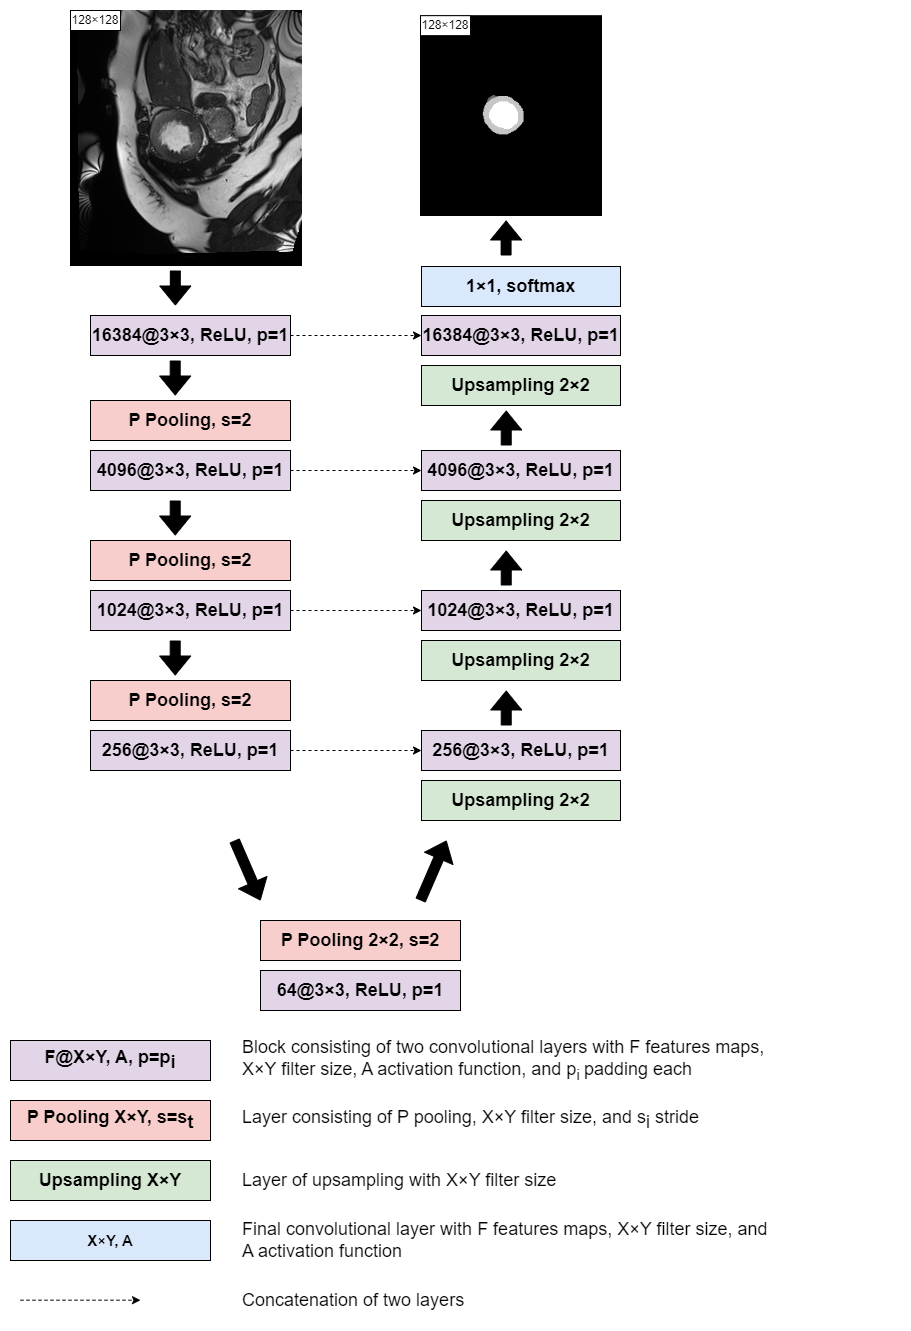
\includegraphics[width=0.86\textwidth]{bab4/ch4-fuzzy-integration.png}
	\caption{Integration of fuzzy pooling within the encoder of the proposed enhanced U-Net framework \citep{Riandini2023MeMeA}}
	\label{fig:ch4-fuzzy-integration}
\end{figure}

As shown in Figure~\ref{fig:ch4-fuzzy-integration}, each convolutional block is followed by a ReLU activation layer before entering the fuzzy pooling module. The resulting feature maps are subsequently propagated to deeper encoder levels while corresponding high-resolution features are preserved through skip connections and later combined during decoder reconstruction. Since only the pooling operation is modified, all remaining components of the segmentation network remain identical to those of the baseline U-Net. This architectural consistency establishes a controlled experimental setting in which the effect of fuzzy pooling can be directly observed.

While Figure~\ref{fig:ch4-fuzzy-integration} illustrates where fuzzy pooling is incorporated within the network architecture, Figure~\ref{fig:ch4-pooling-comparison} explains how the pooling operation aggregates feature responses during encoder down-sampling. This conceptual illustration facilitates understanding of the difference between conventional max pooling and fuzzy pooling before the mathematical formulation of the proposed pooling operation is introduced.

\begin{figure}[htbp]
	\centering
	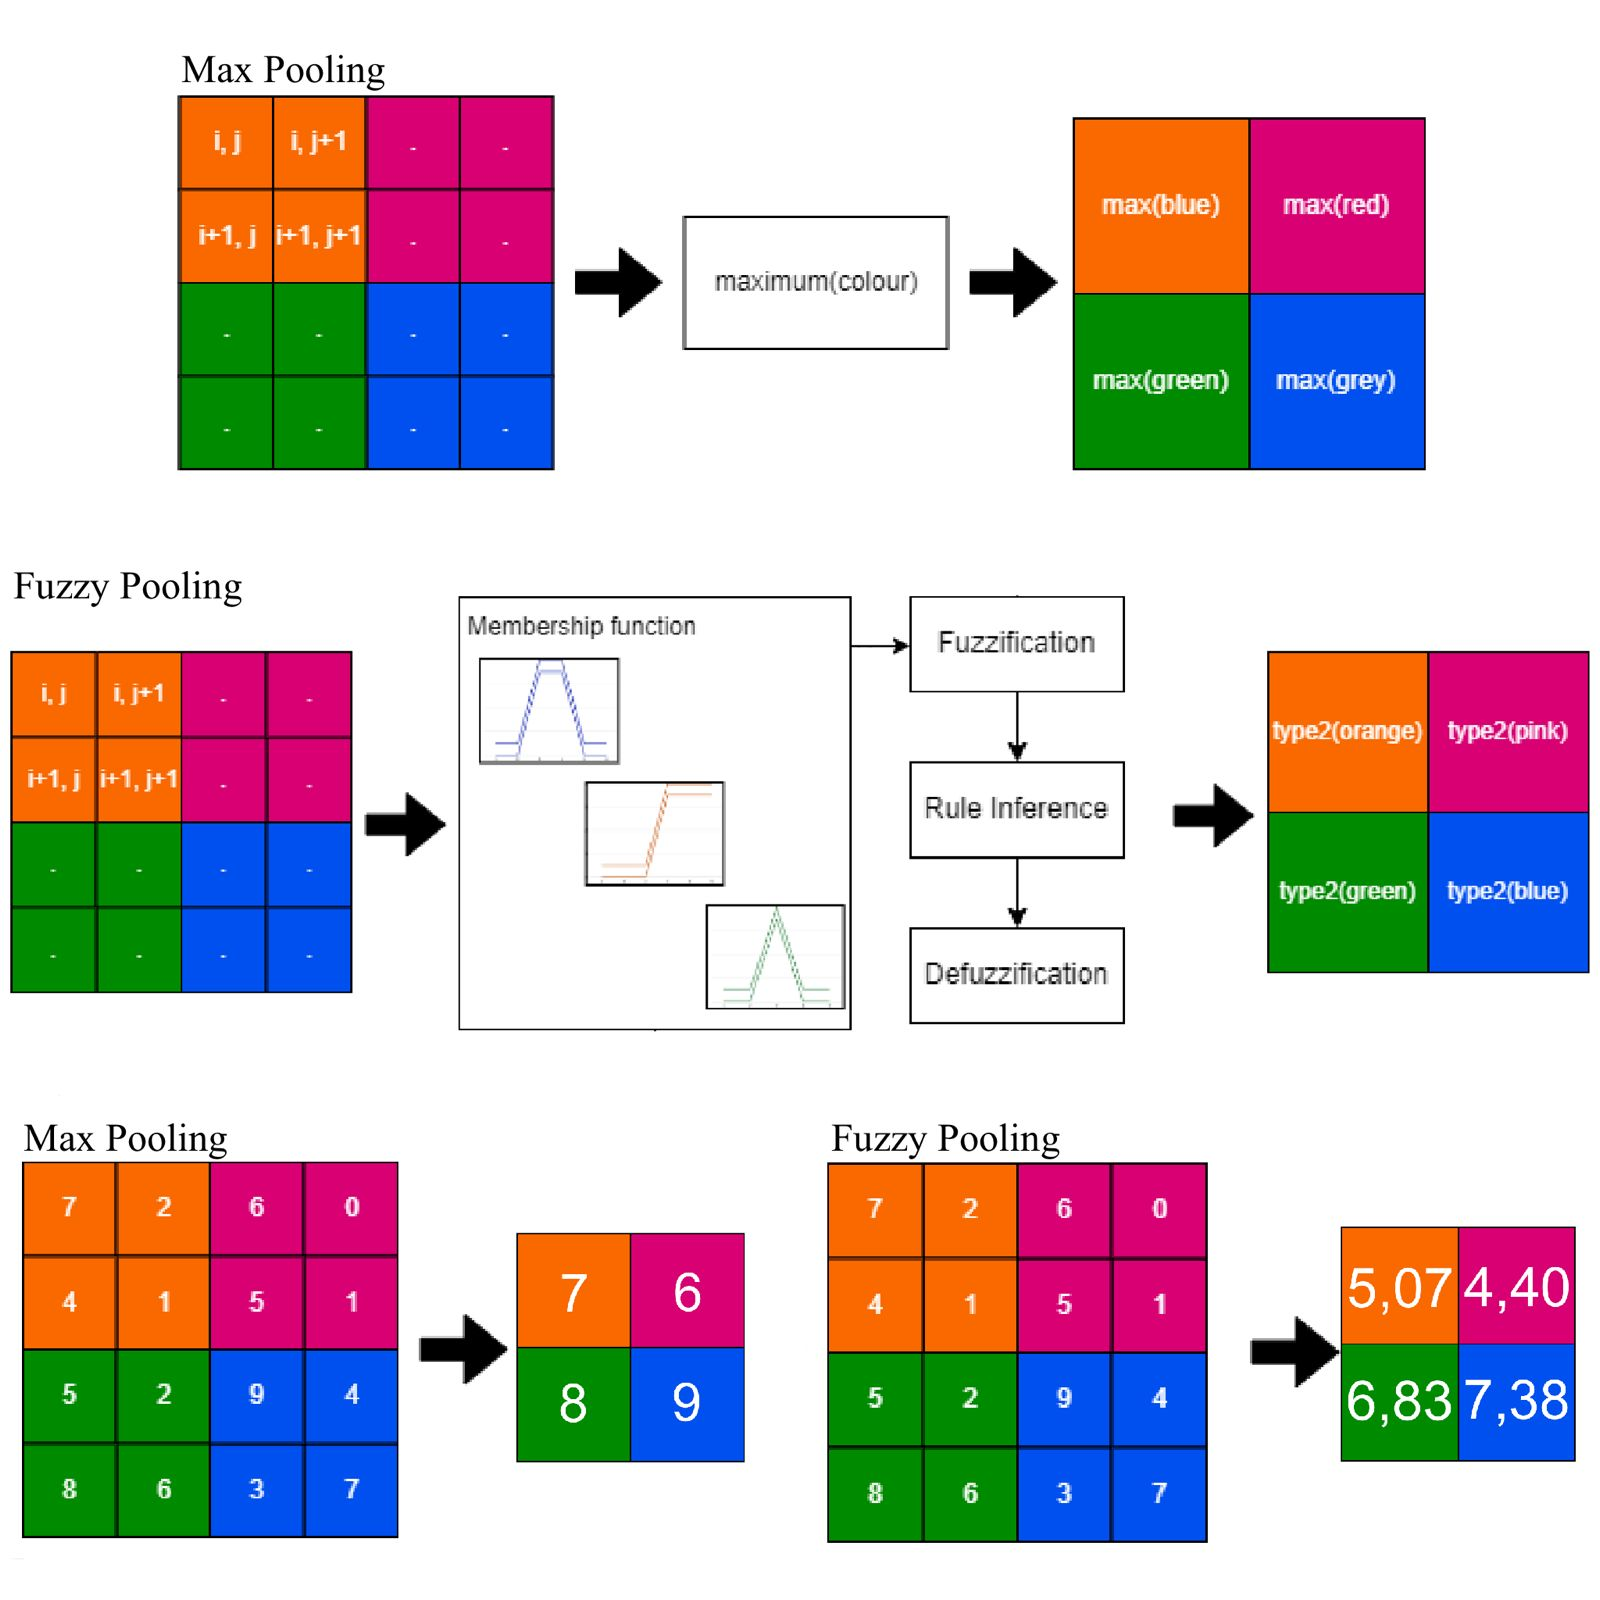
\includegraphics[width=0.86\textwidth]{bab4/ch4-pooling-comparison.png}
	\caption{Illustration of comparison between conventional max pooling and the proposed fuzzy pooling operation \citep{Riandini2023MeMeA}}
	\label{fig:ch4-pooling-comparison}
\end{figure}

Unlike conventional max pooling, which represents an entire pooling region using only its maximum activation, fuzzy pooling evaluates the contribution of every activation within the pooling window through fuzzy membership functions. Instead of selecting a single dominant response, the pooled representation is obtained from the weighted contribution of all neighboring activations according to their relative importance. Consequently, feature aggregation becomes more representative of the local anatomical context rather than depending exclusively on the strongest response.

Based on the feature aggregation mechanism illustrated in Figure~\ref{fig:ch4-pooling-comparison}, the fuzzy pooling operation computes the pooled representation as a weighted combination of all feature responses within the pooling window. The mathematical formulation of the proposed pooling strategy is given by Equation~\eqref{eq:ch4-fuzzy}.

\begin{equation}
	P_{\mathrm{fuzzy}}
	=
	\frac{\sum_{i=1}^{n}\mu_i x_i}
	{\sum_{i=1}^{n}\mu_i}
	\label{eq:ch4-fuzzy}
\end{equation}

where \(x_i\) represents the activation value within the pooling region and \(\mu_i\) denotes its corresponding fuzzy membership coefficient. Unlike max pooling, which ignores all non-maximum activations, this formulation allows informative responses with lower activation values to continue contributing to the encoded feature representation.

From a medical imaging perspective, this characteristic is particularly advantageous for cardiac MRI segmentation. Anatomical boundaries are rarely represented by isolated high-intensity responses; instead, they emerge from spatially correlated intensity transitions distributed across neighboring pixels. By preserving these distributed responses during successive down-sampling operations, fuzzy pooling enables the encoder to retain richer structural information describing ventricular cavities and myocardial boundaries. The decoder subsequently exploits these preserved representations to reconstruct segmentation masks with improved anatomical continuity.

It should be emphasized that the objective of this modification is not to increase network complexity, but rather to improve the quality of hierarchical feature representations learned throughout the encoding process. Therefore, the scientific contribution of this study lies in demonstrating that a relatively simple modification to the feature aggregation mechanism can substantially improve cardiac structure segmentation without requiring additional encoder branches, attention modules, or more complex network architectures.

Collectively, the integration of fuzzy pooling enables improved anatomical feature representation while preserving the original U-Net architecture. This enhanced segmentation framework is subsequently evaluated using the experimental protocol described in the following section.

\section{Materials and Experimental Setup}
\label{sec:ch4-materials}

To objectively evaluate the proposed cardiac structure segmentation framework, a controlled experimental protocol was established to ensure that the observed performance differences originated solely from the investigated pooling mechanism. Accordingly, all comparative models utilized the same dataset, preprocessing procedures, training strategy, and evaluation protocol, thereby enabling the effectiveness of the proposed cardiac structure segmentation framework to be objectively evaluated under controlled and reproducible conditions.

The following subsections describe the dataset, computational environment, training configuration, and evaluation metrics adopted to validate the proposed framework.

\subsection{Dataset}
\label{subsec:ch4-dataset}

The proposed framework was evaluated using the Automated Cardiac Diagnosis Challenge (ACDC) 2017 dataset, one of the most widely adopted public benchmarks for CMR segmentation. The dataset was selected because it provides expert-annotated segmentation masks for the left ventricle (LV), right ventricle (RV), and myocardium (MYO), enabling objective and reproducible evaluation of multi-structure cardiac segmentation algorithms. In addition, the inclusion of multiple cardiac pathologies provides substantial anatomical variability, allowing the robustness of the proposed framework to be assessed under clinically diverse conditions.

The ACDC dataset consists of cine cardiac MRI examinations acquired from 150 patients representing five clinical groups, namely normal subjects, previous myocardial infarction, dilated cardiomyopathy, hypertrophic cardiomyopathy, and abnormal right ventricle. Each examination contains short-axis cine MRI slices covering the cardiac cycle, together with expert manual annotations for the LV, RV, and MYO at the End-Diastole (ED) and End-Systole (ES) phases. These expert annotations serve as the reference standard for supervised training and quantitative evaluation.

Following the experimental protocol adopted in the source study, the dataset was divided into 100 patients for training and 50 patients for testing, resulting in 1,616 training images and 286 testing images after extracting the ED and ES frames from each examination. Using identical data partitions throughout all comparative experiments eliminates dataset-related variability and ensures that the observed performance differences originate from the investigated pooling mechanism rather than differences in data distribution.

Prior to network training, all images were resized to 128 $\times$ 128 pixels while preserving the complete anatomical field of view through image resampling. Pixel intensity normalization was subsequently applied to reduce intensity variation among examinations and to facilitate stable training during network training. The same preprocessing pipeline was consistently applied to all comparative models to ensure fair and reproducible performance evaluation.

\subsection{Experimental Environment}
\label{subsec:ch4-environment}

To ensure reproducibility and experimental consistency, all comparative experiments were conducted under an identical computational environment. Maintaining the same hardware platform, software implementation, preprocessing pipeline, and inference procedure minimizes external sources of variability and ensures that any observed performance differences can be attributed exclusively to the investigated pooling mechanism.

Both the baseline U-Net and the proposed enhanced U-Net were implemented using the Python programming language together with established deep learning libraries for medical image analysis. Model training was performed on a Graphics Processing Unit (GPU), enabling efficient selection of the encoder--decoder architecture and reducing computational time during iterative training.

Throughout the experimental study, the computational environment remained unchanged for all comparative models. Consequently, hardware configuration, software implementation, preprocessing procedures, and inference settings were identical across all experiments. This controlled experimental environment provides a fair basis for comparing the conventional max pooling strategy with the proposed fuzzy pooling approach, ensuring that the reported improvements reflect the effectiveness of the proposed feature aggregation mechanism rather than differences in implementation or computational resources.

\subsection{Training Configuration}
\label{subsec:ch4-training}

A controlled training strategy was adopted to isolate the influence of the pooling mechanism from other selection factors. Therefore, all comparative models utilized the same network architecture, activation function, optimizer, learning rate, training protocol, and stopping criteria. The only architectural modification introduced in this study was the replacement of the conventional max pooling layers with fuzzy pooling throughout the encoder pathway. This controlled configuration ensures that the contribution of fuzzy pooling can be evaluated independently without interference from other training variables.

Except for the batch size required by each pooling strategy, all remaining experimental settings were maintained consistently to ensure a fair comparison between the investigated pooling methods.

The complete experimental settings adopted throughout this study are summarized in Table~\ref{tab:ch4-training}.

\begin{table}[htbp]
	\centering
	\caption{Training configuration}
	\label{tab:ch4-training}
	\begin{tabularx}{0.88\textwidth}{p{0.30\textwidth} X}
		\toprule
		\textbf{Parameter} & \textbf{Configuration} \\
		\midrule
		Dataset & ACDC \\
		Input size & $128 \times 128$ pixels \\
		Activation function & ReLU \\
		Optimizer & Adam \\
		Learning rate & 0.0001 \\
		Batch size & 8 (max pooling); 4 (fuzzy pooling) \\
		Loss function & Categorical cross-entropy \\
		Evaluation metrics & IoU and HD \\
		\bottomrule
	\end{tabularx}
\end{table}

As summarized in Table~\ref{tab:ch4-training}, the principal model and training settings were maintained consistently, except for the batch size specified for each pooling strategy. Consequently, the pooling mechanism remained the principal architectural variable, allowing the observed performance differences to be attributed directly to the proposed fuzzy pooling strategy.

The ReLU activation function was consistently applied throughout all experiments based on the findings of the preliminary investigation presented in the previous chapter. Maintaining the same activation function eliminates selection variability associated with nonlinear feature transformation and ensures that the observed performance differences originate from the investigated pooling mechanism.

\subsection{Evaluation Metrics}
\label{subsec:ch4-metrics}

The segmentation performance of the proposed framework was evaluated using IoU and HD. IoU was used to evaluate the agreement between the predicted segmentation and the corresponding ground-truth annotation, whereas HD was used to assess boundary localization accuracy. The combination of these complementary metrics enables simultaneous evaluation of regional overlap and anatomical contour preservation, both of which are essential for reliable cardiac structure segmentation.

To quantitatively measure the overlap between the predicted segmentation and the corresponding ground-truth annotation, the IoU is computed according to Equation~\eqref{eq:ch4-iou}.

\begin{equation}
	\mathrm{IoU}(P,G)
	=
	\frac{|P\cap G|}{|P\cup G|}
	\label{eq:ch4-iou}
\end{equation}

where \(P\) and \(G\) denote the predicted and reference segmentation regions, respectively.

Although IoU effectively evaluates regional agreement, it does not explicitly measure boundary accuracy. Therefore, HD was additionally used to quantify the maximum distance between the predicted contour and the corresponding ground-truth contour.

Since regional overlap alone cannot fully describe segmentation quality, boundary localization accuracy is further evaluated using the HD, which measures the largest boundary discrepancy between the predicted segmentation and the ground truth. The HD is defined as Equation~\eqref{eq:ch4-hd}.

\begin{equation}
	\mathrm{HD}(P,G)
	=
	\max
	\left(
	\max_{p\in P}\min_{g\in G} d(p,g),
	\;
	\max_{g\in G}\min_{p\in P} d(g,p)
	\right)
	\label{eq:ch4-hd}
\end{equation}

where \(P\) and \(G\) represent the sets of boundary points of the predicted and ground-truth segmentations, respectively, and \(d(\cdot,\cdot)\) denotes the Euclidean distance between two boundary points. 

Using both metrics simultaneously enables segmentation performance to be assessed from complementary perspectives. A higher IoU indicates greater agreement between the predicted and reference regions, whereas a lower HD reflects better boundary agreement between the predicted segmentation and the reference. Since reliable segmentation of ventricular and myocardial boundaries is essential for subsequent quantitative cardiac analysis, the combined use of these metrics provides a more comprehensive evaluation of the proposed framework than either metric alone.

The experimental configuration can be summarized as follows:

\begin{itemize}
	\item \textbf{Dataset:} ACDC cine cardiac MRI dataset.
	\item \textbf{Input image size:} $128 \times 128$ pixels.
	\item \textbf{Segmented structures:} LV, RV, and MYO.
	\item \textbf{Optimizer:} Adam.
	\item \textbf{Evaluation metrics:} IoU and HD.
\end{itemize}

To further investigate the robustness of the proposed framework, all evaluations were performed independently for the End-Diastole (ED) and End-Systole (ES) phases. These two phases exhibit substantially different ventricular morphology and therefore present different levels of segmentation difficulty. Evaluating the proposed framework under both conditions enables a more rigorous assessment of its ability to preserve anatomical structures throughout the cardiac cycle.

\section{Experimental Results and Discussion}
\label{sec:ch4-results}

The effectiveness of the proposed cardiac structure segmentation framework was evaluated through a series of controlled experiments using the ACDC benchmark dataset. As described in Section~\ref{sec:ch4-materials}, all comparative models were developed under controlled experimental conditions, including the dataset, preprocessing pipeline, network architecture, activation function, training strategy, and evaluation protocol. Consequently, the pooling mechanism constituted the principal architectural variable, while the batch size followed the source-study configuration, allowing its contribution to segmentation performance to be objectively assessed.

To provide a comprehensive evaluation, the experimental findings are analyzed from four complementary perspectives. First, the training behaviour of the proposed framework is examined through the learning curves obtained during network training. Second, quantitative segmentation performance is evaluated using the IoU and HD. Third, qualitative comparisons are performed to assess the anatomical consistency of the generated segmentation masks. Finally, the overall findings are synthesized to explain the scientific contribution of the proposed framework and its implication for the subsequent stage of this research.

\subsection{Training Behaviour Analysis}
\label{subsec:ch4-training-behaviour}

Before evaluating the final segmentation accuracy, the convergence behaviour of the proposed framework was first examined to determine whether the integration of fuzzy pooling influences the learning process. Stable convergence indicates that the network is capable of learning representative feature patterns while maintaining good generalization to unseen data, whereas a large discrepancy between the training and validation losses may indicate overfitting. Therefore, analysing the learning behaviour provides an initial assessment of the effectiveness of the proposed feature aggregation strategy. The corresponding training and validation loss curves obtained during the training process are presented in Figure~\ref{fig:ch4-loss-curves}.

\begin{figure}[htbp]
	\centering
	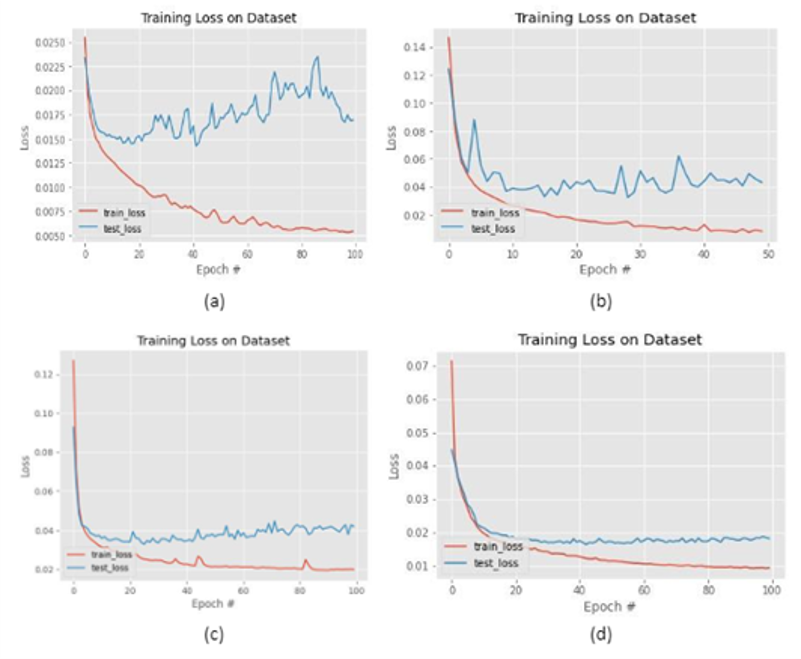
\includegraphics[width=0.86\textwidth]{bab4/ch4-loss-curves.png}
	\caption{Training and validation loss curves obtained using different pooling mechanisms and loss functions \citep{Riandini2023MeMeA}}
	\label{fig:ch4-loss-curves}
\end{figure}

Figure~\ref{fig:ch4-loss-curves} shows that all models successfully converged during the training process. Nevertheless, noticeable differences can be observed between the conventional U-Net adopting max pooling and the proposed framework incorporating fuzzy pooling, particularly for the multi-class segmentation task.

For the model using conventional max pooling with categorical cross-entropy, the training loss decreases rapidly, whereas the validation loss remains consistently higher throughout the training process. The relatively large gap between the two curves indicates that the learned feature representations are more strongly adapted to the training data, thereby reducing the model's ability to generalize to previously unseen cardiac MRI images.

In contrast, the proposed framework adopting fuzzy pooling demonstrates a more stable training behaviour. The training and validation losses decrease simultaneously with a noticeably smaller separation between the two curves, indicating that the learned feature representations are more robust and less sensitive to variations between the training and testing data. This behaviour suggests that preserving richer contextual information during feature aggregation contributes to a more effective learning process.

The convergence patterns observed in Figure~\ref{fig:ch4-loss-curves} are further supported by the final loss values summarized in Table~\ref{tab:ch4-loss}. While the learning curves provide a visual representation of the training process, the numerical results facilitate a more objective comparison between the conventional max pooling and the proposed fuzzy pooling strategies.

\begin{table}[htbp]
	\centering
	\caption{Final loss values obtained using different pooling mechanisms and loss functions}
	\label{tab:ch4-loss}
	\begin{tabular}{l l c}
		\toprule
		\textbf{Pooling mechanism} & \textbf{Loss function} & \textbf{Final loss} \\
		\midrule
		Max pooling & Binary cross-entropy & 0.01783 \\
		Fuzzy pooling & Binary cross-entropy & 0.04680 \\
		Max pooling & Categorical cross-entropy & 0.03596 \\
		Fuzzy pooling & Categorical cross-entropy & 0.03225 \\
		\bottomrule
		\multicolumn{3}{@{}l}{\vspace{4pt}\footnotesize \textit{Source:} Adapted from \citet{Riandini2023MeMeA}.}
	\end{tabular}
\end{table}

As summarized in Table~\ref{tab:ch4-loss}, the effectiveness of the pooling mechanism depends on the segmentation objective. For binary segmentation using binary cross-entropy, the conventional max pooling model achieved a lower loss value (0.01783) than the fuzzy pooling model (0.04680).

A different trend is observed for multi-class segmentation using categorical cross-entropy, which represents the primary objective of this study. The proposed fuzzy pooling model achieved a lower loss value (0.03225) than the conventional max pooling model (0.03596). This corresponds to a reduction of 0.00371, or approximately 10.3\%, indicating that the proposed framework learns more representative feature distributions for multi-class cardiac structure segmentation than the baseline architecture.

Although the numerical reduction appears relatively small, its scientific significance should be interpreted within the context of the experimental design. Both models were trained using identical datasets, preprocessing procedures, activation functions, training algorithms, and learning rates. Therefore, the lower loss obtained by the proposed framework can reasonably be attributed to the integration of fuzzy pooling rather than differences in training settings or network architecture.

The improved training performance can be attributed to the feature aggregation mechanism introduced by fuzzy pooling. Unlike conventional max pooling, which preserves only the strongest activation within each pooling region, fuzzy pooling aggregates information from multiple neighboring activations according to their relative contributions. Consequently, richer contextual information is retained during encoder down-sampling, enabling the network to learn more representative anatomical features.

Overall, the training behaviour analysis demonstrates that integrating fuzzy pooling contributes to more stable convergence and improved feature learning during network training. The agreement between the learning curves and the final loss values indicates that the proposed framework learns more representative anatomical features, which subsequently lead to improved cardiac structure segmentation performance. The quantitative segmentation results are presented in the following subsection.

\subsection{Quantitative Segmentation Performance}
\label{subsec:ch4-quantitative}

The effectiveness of the proposed cardiac structure segmentation framework was quantitatively evaluated using two complementary metrics, namely IoU and HD. IoU measures the degree of overlap between the predicted segmentation and the manually annotated reference, whereas HD evaluates the maximum boundary discrepancy between the corresponding contours. Evaluating both metrics simultaneously provides a comprehensive assessment of segmentation quality because reliable cardiac structure segmentation requires not only accurate region identification but also precise anatomical boundary delineation.

The quantitative comparison between the conventional U-Net using max pooling and the proposed enhanced U-Net incorporating fuzzy pooling is presented in Table~\ref{tab:ch4-performance}.

\begin{table}[htbp]
	\centering
	\caption{Quantitative comparison between max pooling and fuzzy pooling}
	\label{tab:ch4-performance}
	\begin{tabular}{l c c c c}
		\toprule
		\textbf{Pooling} & \textbf{IoU ED (\%)} & \textbf{IoU ES (\%)} & \textbf{HD ED} & \textbf{HD ES} \\
		\midrule
		Max pooling & 90.690 & 74.500 & 6.3249 & 4.2426 \\
		Fuzzy pooling & 93.429 & 85.802 & 3.0000 & 3.1622 \\
		\midrule
		Improvement & +3.0\% & +15.2\% & 52.6\% lower & 25.5\% lower \\
		\bottomrule
	\multicolumn{3}{@{}l}{\vspace{4pt}\footnotesize \textit{Source:} Adapted from \citet{Riandini2023MeMeA}.}
	\end{tabular}
\end{table}

The numerical results summarized in Table~\ref{tab:ch4-performance} demonstrate that replacing conventional max pooling with fuzzy pooling consistently improves segmentation performance from both regional overlap and boundary localization perspectives. Compared with the baseline, IoU increased from 90.690\% to 93.429\% during the End-Diastole (ED) phase and from 74.500\% to 85.802\% during the End-Systole (ES) phase, corresponding to relative improvements of approximately 3.0\% and 15.2\%, respectively.

A similar trend is observed for boundary localization accuracy. The Hausdorff Distance decreased from 6.3249 to 3.0000 during the ED phase and from 4.2426 to 3.1622 during the ES phase, representing reductions of approximately 52.6\% and 25.5\%, respectively. These lower HD values indicate that the predicted cardiac contours more closely match the manually annotated reference boundaries.

Taken together, the improvements observed in both IoU and HD demonstrate that the proposed framework achieves more accurate segmentation not only in terms of regional overlap but also in anatomical boundary localization. The complementary behavior of these two evaluation metrics indicates that incorporating fuzzy pooling enhances feature preservation during the encoding process, leading to more reliable segmentation of cardiac structures across both cardiac phases.

The quantitative findings presented in this section are further examined through qualitative visual comparisons in the following section.

\subsection{Qualitative Segmentation Analysis}
\label{subsec:ch4-qualitative}

While the quantitative evaluation presented in the previous section demonstrates that the proposed framework consistently improves segmentation performance, numerical metrics alone are insufficient to explain how these improvements are reflected in the resulting anatomical structures. Therefore, a qualitative analysis was conducted by visually comparing the segmentation masks generated using the conventional U-Net with max pooling and the proposed enhanced U-Net incorporating fuzzy pooling. This analysis provides complementary evidence regarding anatomical consistency, boundary continuity, and the preservation of fine structural details.

To complement the quantitative evaluation presented in the previous subsection, representative segmentation results generated by the conventional U-Net and the proposed enhanced U-Net are visually compared in Figure~\ref{fig:ch4-qualitative}. This comparison enables direct assessment of anatomical consistency and boundary preservation that may not be fully reflected by numerical performance metrics alone.

\begin{figure}[htbp]
	\centering
	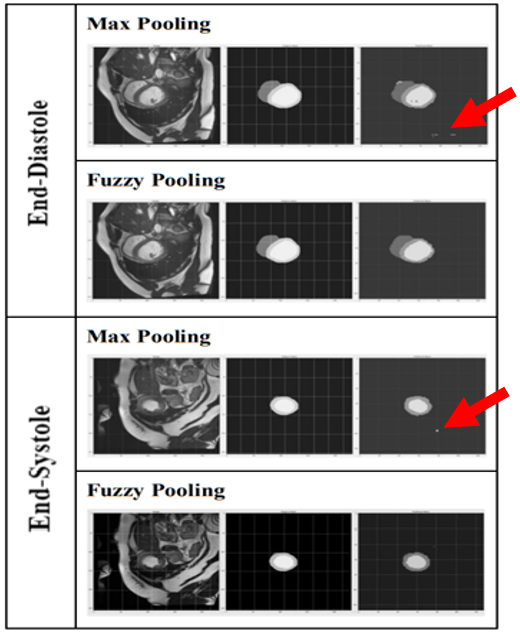
\includegraphics[width=0.86\textwidth]{bab4/ch4-qualitative.png}
	\caption{Qualitative comparison of cardiac structure segmentation obtained using conventional max pooling and the proposed fuzzy pooling for representative End-Diastole and End-Systole images \citep{Riandini2023MeMeA}}
	\label{fig:ch4-qualitative}
\end{figure}

As illustrated in Figure~\ref{fig:ch4-qualitative}, both models successfully identify the major cardiac structures, including the left ventricle (LV), right ventricle (RV), and myocardium (MYO). However, the segmentation produced by the proposed framework exhibits boundaries that more closely follow the expert annotations, indicating improved preservation of anatomical structures during feature extraction and reconstruction. Hence, the structures are observed as: 
%\paragraph{Main observations.}
\begin{itemize}
	\item \textbf{LV:} smoother endocardial contour with fewer boundary irregularities.
	\item \textbf{RV:} improved contour continuity despite its irregular crescent-shaped geometry.
	\item \textbf{MYO:} more uniform myocardial thickness with better preservation of thin anatomical structures.
\end{itemize}

In general, fewer isolated segmentation artifacts and improved anatomical consistency.

The qualitative observations are consistent with the quantitative results presented in Section~\ref{subsec:ch4-quantitative}. The smoother ventricular contours and improved myocardial continuity observed in Figure~\ref{fig:ch4-qualitative} explain the higher Intersection over Union values and lower Hausdorff Distances achieved by the proposed framework. In particular, the substantial reduction in Hausdorff Distance is visually reflected by the improved alignment between the predicted and reference boundaries, whereas the increased IoU corresponds to better overlap of the segmented anatomical regions.

Overall, the qualitative analysis confirms that the proposed framework improves not only numerical segmentation performance but also the anatomical fidelity of the generated segmentation masks. The agreement between the quantitative and qualitative evaluations indicates that integrating fuzzy pooling into the U-Net architecture enhances feature preservation during encoder down-sampling, resulting in more accurate and anatomically consistent cardiac structure segmentation.

\subsection{Overall Discussion}
\label{subsec:ch4-discussion}

The experimental results consistently demonstrate that integrating fuzzy pooling into the encoder of the U-Net architecture improves cardiac structure segmentation without modifying the overall network topology. The improvements observed in both quantitative and qualitative evaluations indicate that preserving richer contextual information during feature aggregation enhances anatomical consistency while reducing boundary errors.

The resulting anatomical myocardium representation established in this chapter provides the structural basis for the subsequent investigations presented in this dissertation. Building upon this framework, Chapter V investigates the influence of different loss functions on myocardium segmentation, whereas Chapter VI extends the analysis toward myocardial scar segmentation and quantitative scar area estimation.

\section{Chapter Summary}
\label{sec:ch4-summary}

This chapter presented an enhanced U-Net framework for cardiac structure segmentation by integrating fuzzy pooling into the encoder pathway. Experimental results demonstrated that the proposed framework improved cardiac structure segmentation compared with the conventional U-Net, providing accurate segmentation of the left ventricle, right ventricle, and myocardium.

The findings demonstrate that preserving richer anatomical information during feature extraction contributes to more accurate cardiac structure segmentation. The resulting anatomical myocardium representation supports the subsequent investigation of loss functions presented in Chapter V and the myocardial scar assessment framework developed in Chapter VI.
